% Propietario conservado: /Users/ruben/Documents/New project/output/EXTREMA_MEDIA_RAZON_RECIPROCIDAD_ES_EN_20260918/ARTICULO/ES/source/sections/excepcional.tex
\section{Exceptional prolongation: from dodecaphasic incidence to Moonshine}
\label{x_reciprocidad:exc:seccion}

The numerical expression does not exhaust the state that generated it. In the
preceding construction, APP preserves the two sheets and division with
remainder and quotient; TRIT determines the local regime and its orientation;
TPK composes selection, transport, carry, memory and return. The
Archimedean reading contracts compatible cylinders. The reading now
studied instead preserves the incidence of positions and its
transport between frames. Both start from the same arithmetic state with
trajectory memory. No
exceptional geometry is reconstructed from the final decimals
of $\pi$, $\varphi$, $e$ or $\alpha$.

This point makes the meaning of the prolongation
$\alpha/K\longrightarrow\text{exceptional incidence}$ precise. The arrow does not
assert that an isolated real number determines a code, lattice or
group. It transports the dodecaphasic register and signed data that
entered into the determination of $\alpha$, together with the words and
frames arising from APP--TRIT--TPK. In particular, the ordered register
$K$ can be recovered from its rational constant $\kappa$ with the
base, length and origin conventions already fixed. Projection onto a
support, by contrast, preserves only the selected incidences.
Meanwhile, $K_{\rm ph}$
denotes another reading, with reduced memory, subsequent to the holonomy
$\Gamma_9$.

The exposition separates three mathematical operations: constructing the finite
objects and their maps; prolonging them to a lattice and a vertex
operator algebra; subsequently recognizing the resulting objects through the relevant
classical theorems. The names Paley, Witt, Mathieu, Golay, Leech and
Monster denote those recognitions and the explicit realizations
making them verifiable. They are not retrospective selectors of the
seeds or coefficients of generation.


% BEGIN OWNER /Users/ruben/Documents/New project/output/EXTREMA_MEDIA_RAZON_RECIPROCIDAD_ES_EN_20260918/ARTICULO/ES/source/sections/revision_incidencia_argumento.tex
The argument starts with compatibility of prefixes and frames,
constructs the ternary code and determines the flag through \(K\) and the
signed register of \(\alpha\). Marked incidence then selects
the lattice origin and Leech neighbor. The final step realizes the vertex
algebra and its automorphisms. At each stage the structure preserved
will be specified: linear combinations, supports, discriminant classes, bilinear
form or graded product. Explanations of the function of \(K\),
normalization and the origin of norm \(54\) accompany their respective
constructions in Sections \ref{x_reciprocidad:exc:bandera} and \ref{x_reciprocidad:exc:leech}.

% END OWNER




\subsection{Compatibility of the Archimedean and incidence realizations}
\label{x_reciprocidad:exc:doble-lectura}

Let $X_n^{\rm cal}$ be the space of admissible prefixes of length $n$ of the
arithmetic state with trajectory memory, with truncations
$p_{n,m}:X_n^{\rm cal}\to X_m^{\rm cal}$ for $m\leq n$. The superscript
recalls that the declared initial frame and its transport are preserved, not
that a parameter is fitted against an experimental value. We write
$(w_j,f_j)$ for the visible word of six trits and the frame at step
$j$. The frames satisfy a causal law
\[
 f_{j+1}=g_j(x)f_j,
\]
where $g_j(x)$ depends on the prefix already constructed. Consequently, a
prolongation does not alter earlier frames.

The chain
\[
 w_6\longrightarrow w_{12}\longrightarrow w_{18}
 \longrightarrow w_{24}\longrightarrow w_{30}
 \longrightarrow R_{36}\longrightarrow G_9
\]
is preserved in this reading. Phase return resets neither the
frame nor the state memory. Likewise, the census of
$468$ decimal emissions, the $243$ visible words of six
trits and the ambient space $\mathbb F_3^6$, of $729$ words, remain distinct. The ambient space
will be used to construct a linear code; it does not replace the admissible
domain of emissions.

For a block $b$ of six trits, the Archimedean reading takes its
integer address $\nu(b)\in\{0,\ldots,728\}$. A prefix determines
\[
 q_n=m+\sum_{j=0}^{n-1}\frac{\nu(b_j)}{729^{j+1}},
 \qquad I_n=[q_n,q_n+729^{-n}].
\]
Prefix compatibility gives nested cylinders whose diameter tends
to zero. Their Cauchy class belongs first to the internal completion
$\mathbb R_{\rm HMT}$; its subsequent identification with the usual real
line does not enter into the choice of blocks.

For the incidence reading we introduce, on the same prefix, the
graph map
\begin{equation}
 \gamma_A:\mathbb F_3^6\longrightarrow\mathbb F_3^{12},
 \qquad w\longmapsto(w,wA).
 \label{x_reciprocidad:exc:gamma}
\end{equation}
Words are written as row vectors. If $A^f=fAf^{-1}$, the
change of frame satisfies the concrete identity
\begin{equation}
 \gamma_{A^f}(wf^{-1})
   =\gamma_A(w)(f^{-1}\oplus f^{-1}).
 \label{x_reciprocidad:exc:covariancia}
\end{equation}
The calibrated codomain preserves $f$ together with the encoded word.
We then define
\begin{equation}
 Q_n(x)=\bigl((f_j,\gamma_{f_jA_Wf_j^{-1}}(w_j))\bigr)_{0\leq j<n}.
 \label{x_reciprocidad:exc:qn}
\end{equation}

\begin{proposition}[Compatibility and prolongation of the incidence reading]
\label{x_reciprocidad:exc:limite-inverso}
If $r_{n,m}$ truncates the encoded sequences, then
\[
 r_{n,m}Q_n=Q_m p_{n,m}.
\]
Therefore, the $Q_n$ determine a unique map $Q_\infty$ between the
respective inverse limits. In each frame, the map preserves exactly
the visible word, since $\operatorname{pr}_1\gamma_A=\operatorname{id}$.
\end{proposition}

\begin{proof}
Two compatible prefixes have the same words and the same
transport operators up to index $m-1$. By induction, they have
the same frames at those indices. The first $m$ components of
\eqref{x_reciprocidad:exc:qn} coincide, proving the square. The universal
property of the inverse limit gives $Q_\infty$. The recovery assertion
is projection onto the first six coordinates of each graph.
\end{proof}

This local injectivity has a precise domain. It does not prove that
$Q_\infty$ recovers all the deep memory of the TPK state if only the
sequence of visible words and frames has been retained. Still less does it
prove injectivity after passing from words to supports.
Moreover, a general change of basis in $\operatorname{GL}_6(\mathbb F_3)$
does not by itself preserve ordinary Hamming weight. In a general
chart, the incidence and metric of the initial chart are also
transported. The support calculations that follow are performed in the declared
Paley chart; monomial relabelings directly preserve their
coordinate interpretation.

\subsection{The finite realization and the ternary code}
\label{x_reciprocidad:exc:paley-codigo}

The elliptic TRIT operator admits the following finite realization in
the six-position chart. These coordinatize the six units
$\{1,2,4,5,7,8\}$ modulo nine, preserved by modular transport.
On $\mathbb P^1(\mathbb F_5)$, once
the order $\infty,0,1,2,3,4$ is declared, let $C$ be the matrix with zero
diagonal, $C_{\infty,a}=C_{a,\infty}=1$ and
$C_{a,b}=\chi(b-a)$ in the five finite positions. Here
$\chi(1)=\chi(4)=1$, $\chi(2)=\chi(3)=-1$ and $\chi(0)=0$.
This is a coordinate realization of the already transported quadratic
structure; identifying the six positions with the projective
line is a chart datum, not a new numerical input into the
generator.

The quadratic sum identities give $C^2=5I_6$. Reducing modulo
three yields
\begin{equation}
 A_W=
 \begin{pmatrix}
 0&1&1&1&1&1\\
 1&0&1&2&2&1\\
 1&1&0&1&2&2\\
 1&2&1&0&1&2\\
 1&2&2&1&0&1\\
 1&1&2&2&1&0
 \end{pmatrix},
 \qquad A_W^2=2I_6=-I_6.
 \label{x_reciprocidad:exc:aw}
\end{equation}
The quadratic equality realizes the elliptic regime; it does not identify the
field $\mathbb F_3$ with an Archimedean realization of the imaginary
unit. These are distinct realizations of a common operator
relation, with their corresponding domains.

\Needspace{8\baselineskip}
\begin{definition}[Code of the dodecaphasic chart]
\label{x_reciprocidad:exc:codigo}
The ternary code associated with \eqref{x_reciprocidad:exc:aw} is
\[
 C_W=\{(w,wA_W):w\in\mathbb F_3^6\}
       \subset\mathbb F_3^{12}.
\]
Its set of hexads is
\[
 \mathcal H=
 \{\operatorname{supp}(c):c\in C_W,
                           \operatorname{wt}(c)=6\}.
\]
\end{definition}

\begin{proposition}[Self-duality, distance and Witt design]
\label{x_reciprocidad:exc:codigo-witt}
The code $C_W$ is self-dual with parameters $[12,6,6]_3$. Its weight
enumerator is
\begin{equation}
 \sum_{c\in C_W}z^{\operatorname{wt}(c)}
   =1+264z^6+440z^9+24z^{12}.
 \label{x_reciprocidad:exc:enumerador}
\end{equation}
The set $\mathcal H$ has $132$ elements and constitutes a system
$S(5,6,12)$: each set of five positions is contained in a
unique hexad.
\end{proposition}

\begin{proof}
The generator matrix $[I_6\mid A_W]$ has rank six and, by symmetry
of $A_W$, satisfies
\[
 [I_6\mid A_W][I_6\mid A_W]^{\mathsf T}
   =I_6+A_W^2=0.
\]
The code is self-orthogonal with dimension half its length and is therefore
self-dual. Finite evaluation of the $3^6$ words gives
\eqref{x_reciprocidad:exc:enumerador}; this is an enumeration over the explicit matrix,
without real values or external targets. In particular, the minimum
distance is six.

If two words of weight six have the same support, among their six
nonzero coordinate ratios one of the signs $1,-1$ appears at
least three times. Subtracting the corresponding multiple would yield
a nonzero word of weight at most three, impossible. Thus a support
corresponds exactly to the pair $\{c,-c\}$ and there are $264/2=132$
supports. If two distinct supports shared five positions,
the same argument would cancel at least three coordinates of a union
of size seven, producing weight at most four. A
quintuple therefore belongs to at most one hexad. Finally,
\[
 132\binom65=792=\binom{12}5,
\]
so it belongs to one and only one.
\end{proof}

The subsequent recognition is the extended ternary Golay code and
the small Witt design \cite{x_reciprocidad:conwaysloane}. The preceding proof explains which object is
recognized. It does not replace the APP--TRIT--TPK genealogy with a search
among known codes.

\subsection{Dodecaphasic flag associated with \texorpdfstring{$K$ and $\alpha$}{K and alpha}}
\label{x_reciprocidad:exc:bandera}


% BEGIN OWNER /Users/ruben/Documents/New project/output/EXTREMA_MEDIA_RAZON_RECIPROCIDAD_ES_EN_20260918/ARTICULO/ES/source/sections/incidencia_registro.tex
\paragraph{Articulation of the regional coordinates and closure incidence.}
\label{x_reciprocidad:inc-ampl-articulacion}
The function of this prolongation is understood through a distinction
between three operations: preserving a register, evaluating a coordinate and
extracting an incidence relation. All three act on information
produced by APP--TRIT--TPK. Their articulation makes explicit the structural
thesis of the article: a numerical realization has an operator
provenance, and certain data from that provenance also admit a
combinatorial and lattice realization. The equations allow both
paths to be followed with their domains and the information remaining in each.

The starting point is the terminal state with its compatible
prolongations. It preserves the residues and quotients of the two APP
sheets, the TRIT regime and orientation, and TPK transport with its memory.
The closure, propagation and self-scale regions are determined in that
domain before their readers establish the coordinates
$\pi,e,\varphi$. At the same time, the oriented register of the twelve
windows determines the signed vector $U$. The subsequent appearance of $K$
comes from the integral transformation proved in
\S\ref{x_reciprocidad:subsec:k-hadamard}:
\begin{equation}
 U=\mathcal H_{12}K,\qquad
 K=\frac14\mathcal H_{12}U,\qquad
 \mathcal H_{12}^{2}=4I_{12}.
 \label{x_reciprocidad:inc-ampl-registro}
\end{equation}
The congruence defining $\mathcal L_H$ guarantees integrality of
the inverse. In this way, $K$ constitutes a reversible coordinatization
of the signed register in the relevant sublattice. Its positions preserve
phase order; its differences $D_3K,D_4K$ preserve transverse
relations; the sum $Q(K)$ determines the uniform component. This
structure explains why the register participates both in numerical
composition and in selection of a boundary configuration.

The periodic evaluation
\[
 K\longmapsto\kappa_{\mathrm{per}}
 =\frac{\sum_{m=1}^{12}K_m1000^{12-m}}{1000^{12}-1}
\]
keeps the twelve blocks recoverable when base, length and phase
origin are fixed. Extracting a support performs a different
operation: it preserves membership of each position in a class defined
by a threshold and groups registers having the same support. The
distinction between these two maps is decisive. The scalar
precision of $\kappa_{\mathrm{per}}$ and the incidence of $B_K$ are two
specific mathematical contents, related through the complete
register from which they arise.


% END OWNER


In the frame inherited from the dodecaphasic register, the data are
\begin{align}
 K={}&(234,543,140,729,659,824,621,\mathtt{058},914,794,146,601),
 \label{x_reciprocidad:exc:k}\\
 w_\pi={}&010211, &w_e={}&201101,\nonumber\\
 w_\varphi={}&121200, &w_{\rm APP}={}&022020.\nonumber
\end{align}
Applying $\gamma_{A_W}$ yields the following incidences:
\begin{align*}
 P_\pi&=\{2,4,5,6,7,8,9,10,11\},\\
 H_e&=\{1,3,4,6,9,10\},\\
 H_\varphi&=\{1,2,3,4,7,9\},\\
 H_{\rm APP}&=\{2,3,5,10,11,12\}.
\end{align*}
The first is the support of a word of weight nine; the other three
are hexads. Through its high-block reading, the register provides
\begin{equation}
 B_K=\{i:K_i\geq729\}=\{4,6,9,10\}=H_e\cap P_\pi.
 \label{x_reciprocidad:exc:bk}
\end{equation}
The integer $729$ here marks a boundary of the declared block
format. It is not identified merely by cardinality with the ternary
ambient space used in \eqref{x_reciprocidad:exc:codigo}. In this specific register, all
integer thresholds between $660$ and $729$ produce the same support:
the support does not recover the threshold or the twelve blocks.

Before carry, the arithmetic route to $\alpha$ preserves the
signed vector
\begin{equation}
 Z_0=(7,297,353,-430,-715,-1199,-3,286,-894,-528,380,663).
 \label{x_reciprocidad:exc:precarry}
\end{equation}
Its negative support is
\begin{equation}
 H^-_\alpha=\{4,5,6,7,9,10\}.
 \label{x_reciprocidad:exc:halpha}
\end{equation}
These signs are not extracted from the decimal expansion of the scalar
$\alpha$; they are preserved in the state preceding its numerical expression.


% BEGIN OWNER /Users/ruben/Documents/New project/output/EXTREMA_MEDIA_RAZON_RECIPROCIDAD_ES_EN_20260918/ARTICULO/ES/source/sections/incidencia_normalizacion.tex
\paragraph{Alpha normalization and its signed configuration.}
\label{x_reciprocidad:inc-ampl-clausura}
The coordinate of $\alpha$ is determined in the positional path through
composition of the regional blocks and dodecaphasic register. Before
positional division, the oriented combination has components
$Z_j=P_j+E_j-\Phi_j-K_j^{\mathrm{per}}$ and the balance with incoming quotient
is $s_j=Z_j+c_{j+1}$. Normalization satisfies
\begin{equation}
 A_j=s_j-1000c_j=Z_j+c_{j+1}-1000c_j,\qquad 0\leq A_j<1000.
 \label{x_reciprocidad:inc-ampl-normalizacion}
\end{equation}
This identity simultaneously preserves the normalized block and the
contribution of the transported quotient. The limit of compatible
prefixes determines the scalar coordinate of the closure. The
signed configuration, in turn, preserves which positions of the
combination before normalization have a negative defect.
In the initial window, that configuration is the vector $Z_0$ of
\eqref{x_reciprocidad:exc:precarry}, and its negative support is $H^-_\alpha$.

Two contents of the same operation are thus defined. Positional
normalization determines a real coordinate through its compatible
remainders and quotients; the negative support determines a
configuration of positions in the cycle of twelve components. The sign
refers to the register balance before normalization. Its incidence
reading remains available because the state preserves that balance
together with the normalized result. This articulation corresponds to the
proved positional path; comparison with the analytic vacancy
operators retains the precise scope established in the chapter on
$\alpha$.

% END OWNER


\begin{proposition}[Agreement of the two flag selectors]
\label{x_reciprocidad:exc:selector-bandera}
Within $\mathcal H$, the support \eqref{x_reciprocidad:exc:halpha} is the unique hexad
$H$ satisfying
\[
 B_K\subset H\subset P_\pi,
 \qquad
 (|H\cap H_e|,|H\cap H_\varphi|,|H\cap H_{\rm APP}|)=(4,3,2).
\]
Thus, the signed reading and incidence reading select the same
flag $B_K\subset H^-_\alpha$.
\end{proposition}

\begin{proof}
The four hexads containing $B_K$ are obtained by adding,
respectively, the pairs
\[
 \{1,3\},\qquad\{2,11\},\qquad\{5,7\},\qquad\{8,12\}.
\]
Only the second and third pairs are contained in $P_\pi$. For the
second, the intersection with $H_\varphi$ has size three and with
$H_{\rm APP}$ size three; it fails the last condition. For the
third, the three intersections have sizes $4,3,2$. This last one
produces precisely the negative support of \eqref{x_reciprocidad:exc:precarry}.
\end{proof}

Both the flag and its marked frame should be retained:
\[
 \mathcal I_*=(B_K\subset H^-_\alpha),\qquad
 \widetilde{\mathcal I}_*
   =(\mathcal I_*;P_\pi,H_e,H_\varphi,H_{\rm APP}).
\]
Union, intersection and difference operations are equivariant
under simultaneous relabeling of the design. The marked class, not the
position numbers taken in isolation, is the transported object.

\begin{lemma}[Origin selected by marked incidence]
\label{x_reciprocidad:exc:origen}
For the preceding frame,
\[
 o_*=(H_e\cap H_\varphi)
           \setminus(H^-_\alpha\cup H_{\rm APP})=\{1\}.
\]
The rule is equivariant under every automorphism applied simultaneously
to the data of $\widetilde{\mathcal I}_*$.
\end{lemma}

\begin{proof}
The first intersection is $\{1,3,4,9\}$. The union subtracted
contains $3,4,9$ and does not contain $1$. Equivariance follows because a
bijection commutes with set operations.
\end{proof}

This origin will select a direction of the lattice neighbor when the
metric $A_2$ and positive chamber are declared. Incidence alone
does not contain that metric. The lattice step will explicitly preserve
both data.


% BEGIN OWNER /Users/ruben/Documents/New project/output/EXTREMA_MEDIA_RAZON_RECIPROCIDAD_ES_EN_20260918/ARTICULO/ES/source/sections/incidencia_bandera.tex
\paragraph{From ternary encoding to the marked flag.}
\label{x_reciprocidad:inc-ampl-bandera}
The regions also provide the codes $w_\pi,w_e,w_\varphi$ and
$w_{\rm APP}$ in the inherited frame. The map
\[
 \gamma_{A_W}:w\longmapsto(w,wA_W)
\]
preserves the six-component word as its first coordinate and adds
its transform by $A_W$. The relation $A_W^2=-I_6$ fixes the
quadratic compatibility of this realization. The next step,
$c\mapsto\operatorname{supp}(c)$, preserves the nonzero positions.
For words of weight six, the support identifies exactly the pair
$\{c,-c\}$, as proved by the minimum distance of the code. In this way,
the quotient by sign produces the hexads, while the complete code
remains available for operations requiring its symbols.

In this chart, the two constructions of the tetrad coincide:
\begin{equation}
 \{i:K_i\geq729\}
 =H_e\cap P_\pi=B_K=\{4,6,9,10\}.
 \label{x_reciprocidad:inc-ampl-cuaterna}
\end{equation}
The left-hand side comes from an integer comparison of the components
of $K$; the right-hand side, from the intersection of the encoded propagation
and closure supports. The threshold belongs to the declared block
chart and remains explicit in the reader's definition. The
complete register preserves the values on which it acts, even when
different thresholds produce the same subset. The equality therefore
expresses compatibility between specified maps.

The support $H^-_\alpha$ completes that tetrad to a hexad. The
condition of membership in the support $P_\pi$, together with the intersection
sizes $(4,3,2)$ relative to $H_e,H_\varphi,H_{\rm APP}$,
selects a unique hexad. The following proofs combine the two
determinations: that obtained through the sign of $Z_0$ and that obtained
through incidence. The result is organized as
\begin{equation}
 \widetilde{\mathcal I}_*
 =\bigl(B_K\subset H^-_\alpha;
         P_\pi,H_e,H_\varphi,H_{\rm APP}\bigr).
 \label{x_reciprocidad:inc-ampl-marco}
\end{equation}
The inclusion is the flag; the four additional supports constitute
its marked frame. Simultaneous permutations transport the frame and
preserve its inclusions and intersections. The relevant information resides
in this transported configuration and its isomorphism class.

The five regions of $\pi$ here recover their internal differentiation.
They share $w_\pi$ as a visible ternary code, but preserve distinct emissions,
signatures and multiplicities. In the binary realization on a
marked dodecad, the transverse region corresponds to the octad whose
intersection with the dodecad is the tetrad; the other four regions
correspond to the lifts of the four hexads of its star. The
negative region is distinguished by $H^-_\alpha$ and the chart order
individualizes the three positive regions. This correspondence preserves
regional roles and the distribution $432+4\cdot144=1008$, while also
realizing the incidence partition $1+4$.

% END OWNER


\subsection{Isometric intertwining of the incidence representations}
\label{x_reciprocidad:exc:entrelazador}

Incidence defines a linear map whose action can be checked
position by position:
\begin{equation}
 I:\mathbb R^{12}\longrightarrow\mathbb R^{\mathcal H},
 \qquad (Iv)(H)=\sum_{p\in H}v_p.
 \label{x_reciprocidad:exc:incidencia}
\end{equation}
Let $V_{11}=\mathbf1^\perp\subset\mathbb R^{12}$. The two Euclidean
realizations are here subsequent languages for the same finite design.

\begin{proposition}[Isometry of the dodecaphasic screen]
\label{x_reciprocidad:exc:isometria}
We have
\[
 I^{\mathsf T}I=36I_{12}+30J_{12},
\]
where $J_{12}$ is the all-ones matrix. Consequently,
\[
 U_W=\frac16 I\big|_{V_{11}}:
 V_{11}\xrightarrow{\ \sim\ }E_{\rm inc}:=I(V_{11})
\]
is an equivariant isometry for the permutation actions of the
design automorphisms.
\end{proposition}

\begin{proof}
Each point belongs to
$r=\binom{11}{4}/\binom54=66$ hexads, and each pair to
$\lambda_2=\binom{10}{3}/\binom43=30$. These are, respectively, the
diagonal and off-diagonal entries of $I^{\mathsf T}I$. On
$\mathbf1^\perp$, the $J_{12}$ term vanishes, leaving $36I$.
Finally, if $g$ is an automorphism, $p\in H$ is equivalent to
$g(p)\in g(H)$; hence $I\rho_{12}(g)=\rho_{\mathcal H}(g)I$.
\end{proof}

Incidence information also has a specific spectral
reading. Define
\[
 G_{H,H'}=\binom{|H\cap H'|}{4}.
\]

\Needspace{8\baselineskip}
\begin{lemma}[Action of the intersection kernel]
\label{x_reciprocidad:exc:espectro}
If $J_{132,12}$ is the rectangular all-ones matrix,
\[
 GI=30I+15J_{132,12}.
\]
Thus $G$ acts by the scalar $30$ on $E_{\rm inc}$.
\end{lemma}

\begin{proof}
The entry $(H,p)$ of $GI$ counts pairs $(T,H')$ with
$T\subset H\cap H'$, $|T|=4$ and $p\in H'$. If $p\in H$, there are ten
tetrads $T$ containing $p$, each contained in four hexads,
and five not containing it, each with a unique extension of the
quintuple $T\cup\{p\}$. The total is $10\cdot4+5=45$.
If $p\notin H$, the fifteen tetrads of $H$ give one extension each:
the total is $15$. Hence the identity. The rectangular term
vanishes on $V_{11}$.
\end{proof}

Here a material intertwiner does exist: it has a determined domain, codomain,
entries and normalization. For example, any orthogonal
projector $P$ already constructed on $V_{11}$ is transported to
$Q=U_WPU_W^*$ on $E_{\rm inc}$, with
$U_WP=QU_W$. This assertion does not identify all operators
acting on those spaces by their trace alone.


% BEGIN OWNER /Users/ruben/Documents/New project/output/EXTREMA_MEDIA_RAZON_RECIPROCIDAD_ES_EN_20260918/ARTICULO/ES/source/sections/k_direccion_dimensional.tex
\subsection{The direction selected by the dodecaphasic register}
\label{x_reciprocidad:exc:k-direccion}

The register \(K\) has a geometric function complementing its
rational evaluation and support reading. Once the representation
of the twelve positions is constructed, its components determine a
direction in the space of zero-mean variations. The reduction
\(12\to11\) removes the uniform mode; the next reduction
\(11\to10\) removes the direction selected by the register itself.
The two operations therefore have different antecedents.

To declare the chart used completely, consider the group
\(A_5\) of even permutations of five objects and the subgroup
\(C_5=\langle(1\,2\,3\,4\,5)\rangle\). The twelve left cosets
\(r_pC_5\) are ordered by these representatives, written as
lists of images:
\[
\begin{array}{c|c@{\qquad}c|c}
p&r_p&p&r_p\\ \hline
1&(4,3,5,2,1)&7&(5,4,3,2,1)\\
2&(4,2,1,3,5)&8&(1,3,4,2,5)\\
3&(1,2,4,5,3)&9&(4,2,3,5,1)\\
4&(2,5,3,4,1)&10&(3,2,5,4,1)\\
5&(4,3,1,5,2)&11&(4,5,2,3,1)\\
6&(5,1,2,3,4)&12&(5,3,2,4,1).
\end{array}
\]
The action by left multiplication defines an orthogonal
representation \(\rho:A_5\to O(\RR^{12})\):
\(\rho(a)e_p=e_q\) when \(ar_pC_5=r_qC_5\).
This representation chart acts on the register already obtained;
the group characters are not used to choose its twelve values.

Let \(\chi_3\) be the values of the three-dimensional character
\[
\begin{array}{c|ccccc}
\text{class}&1&2^2&3&5_a&5_b\\ \hline
\chi_3&3&-1&0&(1+\sqrt5)/2&(1-\sqrt5)/2.
\end{array}
\]
The class \(5_a\) contains the displayed generator of \(C_5\), and
\(5_b\) contains its square. This convention distinguishes the two
conjugate three-dimensional sectors of the representation. Define
\begin{equation}
 P_3=\frac3{60}\sum_{a\in A_5}\chi_3(a^{-1})\rho(a),
 \qquad P_{11}=I_{12}-\frac1{12}J_{12}.
 \label{x_reciprocidad:eq:k-proyectores-incidencia}
\end{equation}
Both matrices are determined by finite sums in
\(\QQ(\sqrt5)\). The appearance of this quadratic field belongs
to the realization of the representation, subsequent to regional
generation of \(\varphi\).

\begin{lemma}[Projection of the register onto the three-dimensional sector]
\label{x_reciprocidad:lem:k-sector-no-nulo}
We have
\[
 P_3=P_3^{\mathsf T}=P_3^2,\quad
 P_3\mathbf1=0,\quad \operatorname{tr}P_3=3,
 \qquad P_3P_{11}=P_{11}P_3=P_3.
\]
For the register \eqref{x_reciprocidad:exc:k}, the vector
\begin{equation}
 u_K=P_3P_{11}K
 \label{x_reciprocidad:eq:k-vector-direccional}
\end{equation}
is nonzero. Its exact norm is
\begin{equation}
 \lVert u_K\rVert^2
 =\frac{6638585+2275584\sqrt5}{20}>0.
 \label{x_reciprocidad:eq:k-norma-direccion}
\end{equation}
\end{lemma}
\begin{proof}
The character sum in \eqref{x_reciprocidad:eq:k-proyectores-incidencia} is the
isotypic projector. The real character and substitution \(a\mapsto a^{-1}\)
give symmetry. The multiplicity of the sector in the action on
\(A_5/C_5\) is the dimension of its vectors fixed by \(C_5\),
\[
 \frac15\left(3+2\frac{1+\sqrt5}{2}
                 +2\frac{1-\sqrt5}{2}\right)=1.
\]
Hence the rank is three. Its orthogonality to the trivial character
gives \(P_3\mathbf1=0\) and both compositions with \(P_{11}\).
These identities can also be verified by multiplying the
matrices of the finite sum.

Finally, \(\sum K_p=6263\) and substitution of the twelve
components into that same sum gives
\[
 \lVert u_K\rVert^2=K^{\mathsf T}P_3K
 =\frac1{20}\sum_{a\in A_5}
                \chi_3(a^{-1})K^{\mathsf T}\rho(a)K
 =\frac{6638585+2275584\sqrt5}{20}.
\]
This is an exact evaluation of sixty specified terms,
reproduced by the attached certificate with quadratic rational
arithmetic. The two positive coefficients prove nonvanishing.
\end{proof}

\begin{definition}[Dodecaphasic direction and transverse complement]
The direction selected by \(K\) in the declared chart is
\(\ell_K=\RR u_K\). Its transverse complement within
\(V_{11}=\mathbf1^\perp\) is
\[
 V_{10}(K)=V_{11}\cap u_K^\perp.
\]
\end{definition}

\begin{proposition}[Orthogonal reduction determined by \(K\)]
\label{x_reciprocidad:prop:k-reduccion-diez}
The operator
\begin{equation}
 P_{10}(K)=P_{11}
       -\frac{u_Ku_K^{\mathsf T}}{\lVert u_K\rVert^2}
 \label{x_reciprocidad:eq:k-proyector-diez}
\end{equation}
is the orthogonal projector of rank ten onto \(V_{10}(K)\). We have
\[
 V_{11}=\ell_K\mathbin{\oplus^{\perp}}V_{10}(K),
 \qquad P_{10}P_{11}=P_{10},\quad P_{10}u_K=0.
\]
\end{proposition}
\begin{proof}
Let \(E_K=u_Ku_K^{\mathsf T}/\lVert u_K\rVert^2\). The
proved nonvanishing guarantees that it is defined. It is symmetric,
\(E_K^2=E_K\), has rank one and, since \(u_K\in V_{11}\),
\(P_{11}E_K=E_KP_{11}=E_K\). Hence
\[
 (P_{11}-E_K)^2=P_{11}-2E_K+E_K=P_{11}-E_K.
\]
Its image is \(V_{11}\cap u_K^\perp\) and its trace is
\(11-1=10\). The decomposition and remaining identities are
obtained by projection onto the two orthogonal summands.
\end{proof}

This result makes precise a role of \(K\) not exhausted by its designation
as a register: besides reversibly representing oriented
data and selecting the tetrad \(B_K\), it determines a
linear polarization. The direction depends on the complete register through
\(P_3K\), not merely on the four points of its support.
The order of register, representation, direction, and dimensional
reduction has thus been retained (Proposition~\ref{x_reciprocidad:prop:k-reduccion-diez}).

The transformation has a precise covariance law. If the chart is changed
simultaneously by an orthogonal permutation matrix \(S\),
\(K'=SK\) and \(P'_3=SP_3S^{-1}\), then
\[
 u_{K'}'=Su_K,\qquad P'_{10}(K')=SP_{10}(K)S^{-1}.
\]
On the other hand, replacing \(u_K\) with \(a u_K\), with \(a\ne0\),
does not change \(E_K\). The direction retains a polarization and does not
by itself allow recovery of either the amplitude of \(u_K\) or the
complete register. Reversibility of \(\kappa\leftrightarrow K\)
remains in its own domain.

The geometric realization established here is a reduction of spaces
with an inner product. Its subsequent use as a compact direction
requires transporting this line to the corresponding physical realization.
Section \ref{x_reciprocidad:exc:pantallas-dualidad} presents the algebraic map
keeping this reduction and the lattice screen coordinated.

% END OWNER


\subsection{The Witt star and the generation of \texorpdfstring{$M_{12}$}{M12}}
\label{x_reciprocidad:exc:estrella}

\begin{definition}[Star on a tetrad]
\label{x_reciprocidad:exc:def-estrella}
For $B\in\binom{[12]}4$, the Witt star is the family of the
four hexads containing $B$. Its petals are the pairs $H\setminus B$.
The permutation $\sigma_B$ fixes $B$ and exchanges the two points of each
petal.
\end{definition}

The existence of four hexads follows from
\[
 \lambda_4=\frac{\binom81}{\binom21}=4.
\]
Two petals cannot share a point, since two hexads would then
contain the same five-element set. They are therefore four disjoint pairs
partitioning $[12]\setminus B$. This description is neither a five-pointed
star nor a geometric metaphor: it is a four-to-one incidence
of the design.

\begin{figure}[htbp]
\centering
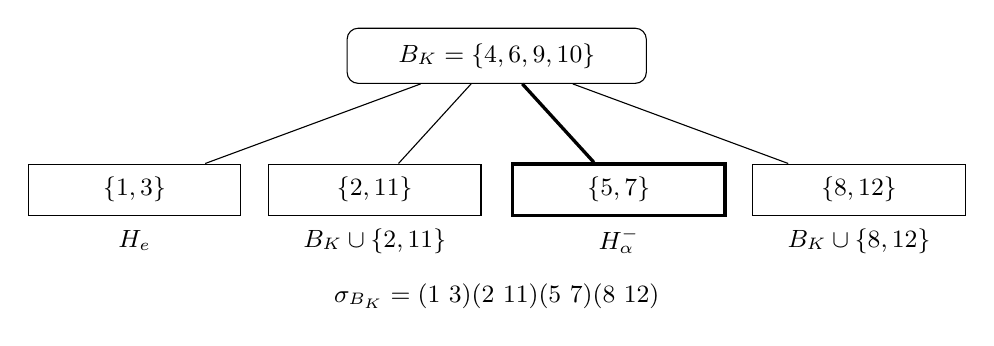
\begin{tikzpicture}[x=1cm,y=1cm, every node/.style={font=\small}]
 \node[draw,rounded corners,minimum width=3.8cm,minimum height=.7cm]
  (b) at (0,0) {$B_K=\{4,6,9,10\}$};
 \node[draw,minimum width=2.7cm,minimum height=.65cm]
  (p1) at (-4.6,-1.7) {$\{1,3\}$};
 \node[draw,minimum width=2.7cm,minimum height=.65cm]
  (p2) at (-1.55,-1.7) {$\{2,11\}$};
 \node[draw,very thick,minimum width=2.7cm,minimum height=.65cm]
  (p3) at (1.55,-1.7) {$\{5,7\}$};
 \node[draw,minimum width=2.7cm,minimum height=.65cm]
  (p4) at (4.6,-1.7) {$\{8,12\}$};
 \draw (b) -- (p1); \draw (b) -- (p2);
 \draw[very thick] (b) -- (p3); \draw (b) -- (p4);
 \node at (-4.6,-2.35) {$H_e$};
 \node at (-1.55,-2.35) {$B_K\cup\{2,11\}$};
 \node at (1.55,-2.35) {$H^-_\alpha$};
 \node at (4.6,-2.35) {$B_K\cup\{8,12\}$};
 \node at (0,-3.05)
  {$\sigma_{B_K}=(1\ 3)(2\ 11)(5\ 7)(8\ 12)$};
\end{tikzpicture}
\caption{The concrete star of the dodecaphasic flag. Each line
indicates the union of the central four-element set with the pair at its endpoint; the
thick line marks the hexad also selected by the signs
preceding the carry of $\alpha$. The four pairs exhaust the eight
outer positions.}
\label{x_reciprocidad:exc:fig-estrella}
\end{figure}

\begin{proposition}[The family of stars]
\label{x_reciprocidad:exc:m12}
The $\binom{12}4=495$ permutations $\sigma_B$ preserve $\mathcal H$.
The group they generate has order $95040$ and is the Mathieu group
$M_{12}$ in its action on the small Witt design.
\end{proposition}

\begin{proof}
The preservation assertion is a finite check on the
$132$ hexads of \eqref{x_reciprocidad:exc:codigo}: for each tetrad the
four petals are constructed and
$\{\sigma_B(H):H\in\mathcal H\}=\mathcal H$ is verified.
Closure under composition of these permutations produces $95040$
elements. In lexicographic enumeration it suffices to add successively
six stars not yet contained in the group; the intermediate orders
are $2,6,18,360,7920,95040$, and the $495$ stars belong to the final
group. The procedure, the six permutations written as their
lists of images and the closure recurrence are developed in
\ref{iv:iv:apendice-estrellas}. Finally, recognition of
the automorphism group of $S(5,6,12)$ as $M_{12}$, whose order is
$12\cdot11\cdot10\cdot9\cdot8=95040$, is applied.
\end{proof}

An individual star generates a cyclic group of order two. It does not
by itself generate $M_{12}$, still less the Monster. Nor does the
existence of $495$ generators of a permutation group prove that
each is the transport of a specific TPK loop. That assertion
requires the corresponding loop map; the result established here
is the finite incidence action.

\begin{remark}[Equality of traces does not identify operators]
On $V_{11}$, a star has spectrum $+1$ with multiplicity seven
and $-1$ with multiplicity four. Its normalized trace is $3/11$.
A rank-three projector on the same space also has normalized
trace $3/11$, but spectrum $1^3,0^8$. They are not conjugate: their
minimal polynomials and spectra differ. The intertwiner
\eqref{x_reciprocidad:exc:incidencia} transports defined operators; it does not turn
this scalar coincidence into an equivalence of operators.
\end{remark}

\subsection{The binary residue and the five regions of \texorpdfstring{$\pi$}{pi}}
\label{x_reciprocidad:exc:cinco-regiones}

The next recognition uses the extended binary Golay code
$G_{24}$, with parameters $[24,12,8]_2$. Its weights are
$0,8,12,16,24$, and the weight-eight supports form the design
$S(5,8,24)$. Fix a dodecad $D$, the support of a word of weight
twelve. This datum and the incidence isomorphism to be declared
below belong to the realization chart; they are not used to
generate or select the decimals of $\pi$.

\begin{proposition}[Residue of a dodecad and lifting of hexads]
\label{x_reciprocidad:exc:residuo-binario}
The set
\[
 \mathcal H(D)=
 \{O\cap D: O\text{ is an octad},\ |O\cap D|=6\}
\]
is an $S(5,6,12)$ system on $D$. Each of its hexads has
a unique lift to an octad. For any four-element set $B\subset D$,
the five octads containing it split into four residual
lifts and a unique octad $O_B^\perp$ with $O_B^\perp\cap D=B$.
\end{proposition}

\begin{proof}
A quintuple $A\subset D$ belongs to a unique octad $O$. If
$j=|O\cap D|$, the binary word given by the sum of $O$ and $D$ has weight
$20-2j$. Among the allowed weights, and with $0\leq j\leq8$, only
$j=2,4,6$ are possible. Since $A\subset O\cap D$, we have $j\geq5$
and therefore $j=6$. This gives existence and uniqueness of the residual
hexad, as well as uniqueness of its lift on choosing five of its
points. Furthermore,
\[
 \lambda_4(S(5,8,24))=\frac{\binom{20}1}{\binom41}=5,
 \qquad
 \lambda_4(S(5,6,12))=4.
\]
The four residual hexads on $B$ give four distinct octads.
The fifth cannot meet $D$ in six points, since it would be another residual
hexad; as it contains $B$, its intersection has size four and
coincides with $B$.
\end{proof}

A chart $\ell:[12]\to D$ preserving hexads identifies
$\mathcal H$ with $\mathcal H(D)$. Its existence is recognition
of the already constructed design as the small Witt design; a specific choice
of $\ell$ fixes the relabeling. The lift
\[
 \iota_D:\mathcal H\longrightarrow
       \{\text{octads of }G_{24}\},
 \qquad H\longmapsto O\text{ such that }O\cap D=\ell(H),
\]
is injective because intersection with $D$ recovers $\ell(H)$.
The domain of this injectivity is the hexads, not the register $K$.

The relation to the five regions of $\pi$ preserves richer data
than the number five. The emissions and their signatures are:
\begin{center}
\small
\begin{tabular}{@{}crll@{}}
\toprule
Region & Multiplicity & Emission $U_6$ & Signature \\
\midrule
$\perp$ & $432$ & $(501,614,498,169,272,272)$ & $555555$ \\
$++_1$ & $144$ & $(810,923,870,169,272,272)$ & $339555$ \\
$++_2$ & $144$ & $(810,983,810,169,272,272)$ & $393555$ \\
$++_3$ & $144$ & $(870,923,810,169,272,272)$ & $933555$ \\
$--$ & $144$ & $(870,923,810,418,674,521)$ & $933717$ \\
\bottomrule
\end{tabular}
\end{center}
In each three-digit decimal block, the signature uses the modular
difference of the first two digits. The five emissions have the
same visible tritic word $w_\pi=010211$, but not the same
regional genealogy. The three positive regions preserve the tail
$169|272|272$; the negative region changes it to $418|674|521$;
the transverse region has constant signature and greater multiplicity.

The marked extension of the regional chart sends the transverse region
to $O_{\ell(B_K)}^\perp$, the negative region to $\iota_D(H^-_\alpha)$ and the
three positive regions to the other three lifts of the star. This
realizes the partition $4+1$ of the five octads on $\ell(B_K)$.
The individual correspondence between the three positive names and
the three remaining petals requires a chart order; incidence does not determine it
without that datum. The precise assertion is therefore a
marked correspondence of regions, compatible with their roles and with
the flag, not a canonical bijection inferred from cardinality five.

The identity $432+4\cdot144=1008$ preserves the regional
multiplicities. Also $1008=36\cdot28$ and an octad has
$\binom82=28$ pairs. These equalities are arithmetic catalogue checks,
not substitutes for the map $\iota_D$ or the regional chart.


% BEGIN OWNER /Users/ruben/Documents/New project/output/EXTREMA_MEDIA_RAZON_RECIPROCIDAD_ES_EN_20260918/ARTICULO/ES/source/sections/estrella_pentadica_recuperada.tex
\subsubsection{Pentadic representation of the microfiber and its incidence}
\label{x_reciprocidad:pi-estrella:desarrollo}

The arrangement of the five regions allows simultaneous visualization
of the unity of the ternary quotient and the differentiation preserved by the
catalogue. The relevant map is the restriction
\[
 \Psi\big|_{\mathscr R_\pi^{\rm micro}}:
 \mathscr R_\pi^{\rm micro}\longrightarrow\{010211\},
 \qquad \Psi(U)=(-U)\bmod3.
\]
Its five antecedents are the vectors \(U_6\) in the preceding table.
Figure \ref{x_reciprocidad:pi-estrella:figura} recovers their radial organization,
preserving chart order, signatures and catalogue
multiplicities (equation~\eqref{x_reciprocidad:eq:palabras-regionales}).


% BEGIN OWNER /Users/ruben/Documents/New project/output/EXTREMA_MEDIA_RAZON_RECIPROCIDAD_ES_EN_20260918/ARTICULO/ES/source/figures/estrella_cinco_regiones.tex
% Orden de carta y datos recuperados de fig_cinco_regiones_pi.tex.
\begin{figure}[H]
\centering
\begin{tikzpicture}[x=1cm,y=1cm,font=\small,>=Latex]
 \coordinate (a) at (90:2.2);
 \coordinate (b) at (18:2.2);
 \coordinate (c) at (-54:2.2);
 \coordinate (d) at (-126:2.2);
 \coordinate (e) at (162:2.2);
 \draw[black!35,line width=.45pt]
    (a)--(c)--(e)--(b)--(d)--cycle;
 \node[draw,fill=white,circle,minimum size=1.6cm,align=center,
    inner sep=3pt] (z) at (0,0) {$w_\pi$\\$010211$};
 \foreach \v in {a,b,c,d,e}{
    \fill (\v) circle (2pt);
    \draw[->,line width=.6pt] (\v)--(z);
 }
 \node[above=3mm,align=center] at (a)
   {$U_\pi^\perp$\\$555555$\\multiplicidad $432$};
 \node[right=3mm,align=left] at (b)
   {$U_{\pi,1}^{++}$\\$339555$\\multiplicidad $144$};
 \node[below right=2mm and 1mm,align=left] at (c)
   {$U_{\pi,2}^{++}$\\$393555$\\multiplicidad $144$};
 \node[below left=2mm and 1mm,align=right] at (d)
   {$U_{\pi,3}^{++}$\\$933555$\\multiplicidad $144$};
 \node[left=3mm,align=right] at (e)
   {$U_\pi^{--}$\\$933717$\\multiplicidad $144$};
 \node[align=center,font=\footnotesize] at (0,-3.55)
   {$1_\perp+3_{++}+1_{--}$\qquad $432+4\cdot144=1008$};
\end{tikzpicture}
\caption{The five regions of \(\pi\) in a pentadic arrangement.
Each position preserves its multiplicative signature and multiplicity;
the radial arrows represent the common projection
\(\Psi(U)=010211\). The star-shaped outline organizes the five
positions of the chart. Their realization in the five Witt octads
is carried out through regional alignment and the decomposition
\(4+1\) in the text.}
\label{x_reciprocidad:pi-estrella:figura}
\end{figure}

% END OWNER


Projection onto the center identifies the five ternary images; the
register of the outer positions retains the regional information
making the incidence realization possible. The distribution
\(1_\perp+3_{++}+1_{--}\) specifies one transverse region, three
positive regions and one negative region. Their normalized weights are
\(3/7\) and \(1/7\) for each of the other four: the
transverse multiplicity is triple, even though the five images under
\(\Psi\) coincide.

\Needspace{11\baselineskip}
The link to the Witt star is formulated through the flag
\(B_K\subset H^-_\alpha\), alignment \(\ell\) and
lift \(\iota_D\) already constructed. The five regional positions
are realized in the five octads on \(\ell(B_K)\):
\[
\begin{aligned}
 U_\pi^\perp&\longmapsto O^\perp_{\ell(B_K)},\\
 U_\pi^{--}&\longmapsto\iota_D(H^-_\alpha),\\
 \{U_{\pi,1}^{++},U_{\pi,2}^{++},U_{\pi,3}^{++}\}
 &\longmapsto
 \{\iota_D(B_K\cup P):P\in\mathcal P_+\},\\
 \mathcal P_+&=\bigl\{\{1,3\},\{2,11\},\{8,12\}\bigr\}.
\end{aligned}
\]
Assignment of the three positive positions to the three pairs is
performed in an ordered chart. The transverse row and negative row
are distinguished by their regional predicates and the flag.

The two figures are thus articulated: Figure
\ref{x_reciprocidad:exc:fig-estrella} shows the four hexads of the small Witt
design on \(B_K\); Figure \ref{x_reciprocidad:pi-estrella:figura} shows
the five regions that, under alignment, occupy the four residual
octads and the transverse octad of the binary design. The law
\(4+1\), proved in Proposition
\ref{x_reciprocidad:exc:residuo-binario}, specifies the incidence change. In this
composition, \(K\) determines the marked tetrad and the signature of
\(\alpha\) distinguishes one of its hexads. In addition to
their common ternary value, the regions preserve the structure needed for that
transport toward the exceptional realization.

% END OWNER


\subsection{From the ternary code to the Niemeier lattice}
\label{x_reciprocidad:exc:niemeier}

The passage to dimension twenty-four does not require first going through the
binary code. It is realized directly from $C_W$ by gluing
discriminants. Two compatible prolongations are thus distinguished:
one preserves the residue $W_{12}\subset W_{24}$; the other constructs the
lattice on which the vertex operator algebra will be realized.

Let $A_2=\mathbb Z a_1\oplus\mathbb Z a_2$ have Gram matrix
\[
 \begin{pmatrix}2&-1\\-1&2\end{pmatrix},
 \qquad \rho=a_1+a_2,\qquad \rho^2=2.
\]
We represent the three classes of $A_2^*/A_2$ by
\[
 \varpi_0=0,\qquad
 \varpi_1=\frac{2a_1+a_2}{3},\qquad
 \varpi_2=\frac{a_1+2a_2}{3}.
\]
The map $j\mapsto\varpi_j+A_2$ additively identifies
$\mathbb F_3$ with that discriminant. For $c\in C_W$, write
$\phi(c)=(\varpi_{c_1},\ldots,\varpi_{c_{12}})$ and define
\begin{equation}
 N(C_W)=\bigcup_{c\in C_W}\bigl(A_2^{12}+\phi(c)\bigr).
 \label{x_reciprocidad:exc:niemeier-def}
\end{equation}

\begin{theorem}[Ternary gluing]
\label{x_reciprocidad:exc:niemeier-teorema}
The object \eqref{x_reciprocidad:exc:niemeier-def} is a positive, even,
unimodular lattice of rank $24$. Its root system is exactly
$A_2^{12}$; it is therefore recognized as the Niemeier lattice with
that root system.
\end{theorem}

\begin{proof}
Linearity of the code makes the union of classes stable under
addition. Self-orthogonality annuls the discriminant pairing:
it is a multiple of $c\cdot d/3$ modulo $\mathbb Z$. Thus the
lattice is integral. The norm of a gluing class is
$2\operatorname{wt}(c)/3$ modulo $2\mathbb Z$. The weights of
\eqref{x_reciprocidad:exc:enumerador} are multiples of three, so it is even.

The index of $A_2^{12}$ in $N(C_W)$ is $|C_W|=3^6$. Consequently,
\[
 \det N(C_W)=\frac{3^{12}}{(3^6)^2}=1.
\]
Positivity comes from the orthogonal sum of the twelve metrics $A_2$.
In a nonzero class of $A_2^*/A_2$ the minimum norm is $2/3$;
every nonzero word has at least six nonzero positions.
Therefore a vector in a nontrivial gluing class has norm
at least $6\cdot2/3=4$. No norm-two roots appear outside
$A_2^{12}$. Inside it, the roots are precisely those of its
twelve components.
\end{proof}

\subsection{Incidence selection of the rootless unimodular neighbor}
\label{x_reciprocidad:exc:leech}


% BEGIN OWNER /Users/ruben/Documents/New project/output/EXTREMA_MEDIA_RAZON_RECIPROCIDAD_ES_EN_20260918/ARTICULO/ES/source/sections/incidencia_reticulo.tex
\paragraph{From the incidence origin to the lattice modification.}
\label{x_reciprocidad:inc-ampl-reticulo}
The marked flag determines a position through an equivariant
set-theoretic operation:
\[
 o_*=(H_e\cap H_\varphi)
       \setminus(H^-_\alpha\cup H_{\rm APP})=\{1\}.
\]
Its function is to distinguish one component among the twelve
involved in the lattice realization. The complete ternary code
acts as a gluing code in the discriminant module
$(A_2^*/A_2)^{12}$. Its preimage defines $N(C_W)$, and the
self-duality, weights and distance of the code translate,
respectively, into integrality and determinant properties, parity
and norm bounds on the gluing classes. Here the symbolic information
of the code serves a function that the isolated support no longer performs.

The metric $A_2$ and positive radial chamber are fixed in the lattice
development. Within that chamber, the congruence required for an even
neighbor of index three has twelve realizations of minimum norm $54$,
permuted by changing the distinguished component. The origin $o_*$
selects
\[
 v_\alpha=4\rho_1+\rho_2+\cdots+\rho_{12},\qquad
 v_\alpha^2=2(4^2+11)=54.
\]
The coefficient $4$ belongs to that solution of the congruence in the
declared chamber. The subscript $\alpha$ records the incidence
provenance of the selection: its content is the frame involved in
closure and now individualizing a lattice direction.

Pairing with $v_\alpha$ determines the sublattice
$N_{\alpha,0}$ of index three, and adding the class
$v_\alpha/3$ produces the neighbor $N_\alpha$ of
\eqref{x_reciprocidad:exc:vecino}. This modification preserves rank and recovers
unimodularity and parity; selection by congruence removes the previous roots,
and local bounds exclude roots in the new classes.
Identification with Leech appears after these verifications. The
binary realization of the five regions and this lattice construction
are two prolongations of the common frame: the latter directly receives
the ternary code as gluing data.


% END OWNER


The label $o_*=1$ of the flag is now realized as one of the
twelve components $A_2$. This operation declares the preceding metric and
the positive radial chamber
\[
 v(a)=\sum_{i=1}^{12}a_i\rho_i,
 \qquad a_i=1+3b_i,\quad b_i\in\mathbb Z_{\geq0}.
\]
The evenness requirement for the index-three neighbor is
$v(a)^2\equiv0\pmod{18}$. Since
\[
 v(a)^2=2\sum_i(1+3b_i)^2,
\]
that congruence is equivalent to $\sum_i b_i\equiv1\pmod3$. The smallest
norm value in the chamber is obtained with a single $b_i=1$ and
all the others zero; it is $54$. The marked origin selects
\begin{equation}
 v_\alpha=4\rho_1+\rho_2+\cdots+\rho_{12},
 \qquad v_\alpha^2=54.
 \label{x_reciprocidad:exc:vector}
\end{equation}
The word ``smallest'' refers to this positive chamber. It does not assert
minimality in the entire residue class: the vector
$(a_1-2a_2,\rho,\ldots,\rho)$ represents the same class modulo three
and has norm $14+11\cdot2=36$. The chamber restriction is part
of the construction data, not an omissible conclusion.

Let $N=N(C_W)$. We define
\begin{equation}
 N_{\alpha,0}=\{x\in N:\langle x,v_\alpha\rangle\equiv0\pmod3\},
 \qquad
 N_\alpha=N_{\alpha,0}+\mathbb Z\frac{v_\alpha}{3}.
 \label{x_reciprocidad:exc:vecino}
\end{equation}

\begin{theorem}[Leech neighbor determined by the marked flag]
\label{x_reciprocidad:exc:teorema-leech}
With the declared metric and chamber, $N_\alpha$ is a positive, even,
unimodular lattice of rank $24$, with no vectors of norm two.
By the corresponding classification theorem, it is isometric to the
Leech lattice $\Lambda_{24}$.
\end{theorem}

\begin{proof}
The character $x\mapsto\langle x,v_\alpha\rangle\bmod3$ is nonzero:
a simple root of one component pairs with $a_i\rho_i$ to give
$a_i\equiv1\pmod3$. Hence $[N:N_{\alpha,0}]=3$ and
$\det N_{\alpha,0}=9$. Moreover,
$v_\alpha/3\in N_{\alpha,0}^*$ and $v_\alpha\in N_{\alpha,0}$.
If $v_\alpha/3$ belonged to $N$, integrality of $N$ would make
all pairings with $v_\alpha$ divisible by three,
contradicting the nonzero character. The class of $v_\alpha/3$ therefore has
order three. We deduce
\[
 [N_\alpha:N_{\alpha,0}]=3,
 \qquad \det N_\alpha=9/3^2=1.
\]
The extension is integral, and for $x\in N_{\alpha,0}$,
\[
 \left(x+m\frac{v_\alpha}{3}\right)^2
   =x^2+2m\frac{\langle x,v_\alpha\rangle}{3}+6m^2
   \in2\mathbb Z.
\]
Hence it is even.

It remains to exclude the roots, which is the decisive step. The roots of $N$
belong to $A_2^{12}$. Their pairings with $v_\alpha$ are
congruent to $\pm1$ or $\pm2$ modulo three; none belongs to
$N_{\alpha,0}$. For the other two classes of the neighbor, each component
belongs to one of the local classes
\[
 A_2+\varpi_j\pm\rho/3,\qquad j=0,1,2.
\]
Since $4\rho/3\equiv\rho/3\pmod{A_2}$, this description also holds
in the distinguished component. Writing a local vector
as $(u a_1+v a_2)/3$, its norm is
$2(u^2-uv+v^2)/9$. The six preceding classes have nonzero residues
and minimum $2/9$: representatives minimizing the quadratic form
are $(\pm1,0),(0,\pm1),(1,1),(-1,-1)$ in the appropriate residues.
A vector in a new class therefore has norm at least
$12\cdot2/9=8/3>2$. There are no roots in any of the three classes.
The classification of positive even unimodular lattices of
rank twenty-four identifies the unique rootless case with
$\Lambda_{24}$.
\end{proof}

The argument does not recognize Leech through a coincidence of dimension.
It constructs the gluing, proves integrality, parity and determinant, and
removes the roots through a local bound. Only then does it apply the
classification theorem. Dependence on $\alpha$ is preserved in
the flag selecting $o_*$ and in the vector \eqref{x_reciprocidad:exc:vector};
the scalar value of the constant is not turned into a lattice
length.

\subsection{The vertex operator algebra and the Monster}
\label{x_reciprocidad:exc:voa}

Let $\Lambda=N_\alpha$, already recognized as Leech. The next step
uses its integral lattice, not a decimal expansion. The lattice
vertex operator algebra construction is written
\[
 V_\Lambda=M(1)\otimes\mathbb C_\varepsilon[\Lambda].
\]
Here $M(1)$ is the Heisenberg oscillator space in rank
twenty-four; $\mathbb C_\varepsilon[\Lambda]$ is the group algebra
twisted by the cocycle of the lattice's central extension. The
cocycle and lift of the isometries are part of the
construction: a bare vector sum does not determine the vertex
products.

Negation $\lambda\mapsto-\lambda$ admits the standard lift
$\theta$. With its twisted module and the compatible parity choice,
the Frenkel--Lepowsky--Meurman construction produces
\begin{equation}
 V^\natural_{\rm HMT}
   =V_\Lambda^+\oplus(V_\Lambda^T)^+.
 \label{x_reciprocidad:exc:flm}
\end{equation}
The sign $+$ denotes the even part of the lifted action. The expression
includes the orbifold vertex product; it is not merely a sum
of graded spaces.

\begin{theorem}[Prolongation to the Moonshine module]
\label{x_reciprocidad:exc:moonshine}
The algebra \eqref{x_reciprocidad:exc:flm}, constructed on the neighbor
\eqref{x_reciprocidad:exc:vecino}, is a realization of the Moonshine algebra
$V^\natural$. It has central charge $24$, zero weight-one component,
and automorphism group isomorphic to the Monster $\mathbb M$. Its graded
character is
\begin{equation}
 \operatorname{Tr}_{V^\natural_{\rm HMT}}q^{L_0-1}
   =J(\tau)=j(\tau)-744
   =q^{-1}+196884q+21493760q^2+\cdots,
 \qquad q=e^{2\pi i\tau}.
 \label{x_reciprocidad:exc:j}
\end{equation}
\end{theorem}

\begin{proof}
Theorem \ref{x_reciprocidad:exc:teorema-leech} verifies the lattice hypotheses:
positivity, parity, unimodularity, rank twenty-four and absence of
roots. The construction and theorem of
Frenkel--Lepowsky--Meurman for the Leech lattice are then applied. They identify
the orbifold with $V^\natural$ and establish its character and automorphism
group. Composition of the flag, neighbor and VOA
construction functor gives the realization indicated here. The group is not
inferred from the coefficient $196884$.
\end{proof}

The theorem used is a subsequent classical recognition with
verified hypotheses, not a new proof in this article of
the FLM construction \cite{x_reciprocidad:flm}.
Moreover, the notation $q=e^{2\pi i\tau}$ is the conventional Fourier
variable used to recognize the character. It introduces neither $\pi$
nor $e$ as inputs to the coinductive generator that has already determined them.

Part of the trace mechanism can be seen before the orbifold.
Only the zero lattice vector is fixed by negation; each
oscillator contributes with alternating sign. Hence
\[
 \operatorname{Tr}_{V_\Lambda}\theta q^{L_0-1}
   =t_2(\tau)
   :=q^{-1}\prod_{n\geq1}(1+q^n)^{-24}.
\]
This trace in the lattice algebra must not be confused with the
character without insertion of $V^\natural$. Nor does it by itself identify
a conjugacy class of the Monster: the space, insertion
and lift must be specified before functions are compared.


% BEGIN OWNER /Users/ruben/Documents/New project/output/EXTREMA_MEDIA_RAZON_RECIPROCIDAD_ES_EN_20260918/ARTICULO/ES/source/sections/incidencia_automorfismos.tex
\paragraph{Grading, unit and automorphisms.}
\label{x_reciprocidad:inc-ampl-automorfismos}
The Frenkel--Lepowsky--Meurman construction is applied to the lattice
$N_\alpha$ once its properties have been verified. It incorporates the oscillator
space, central extension of the lattice, vertex product
and sector twisted by the lift of negation. The result is
the algebra $V^\natural_{\rm HMT}$ of \eqref{x_reciprocidad:exc:flm}, whose automorphism
group is isomorphic to the Monster. Its action domain is thus
fixed by an algebraic structure with grading and product. Borcherds's
Moonshine theorem subsequently determines the graded traces
with insertion of these automorphisms \cite{x_reciprocidad:flm,x_reciprocidad:borcherds}.

Unity acquires a precise realization at this level: the weight-zero
component is the vacuum line and contributes the coefficient $1$ of
$q^{-1}$ in the graded character. At the cylindrical level, the
refinement maps preserve the constant function by
precomposition. Each conservation assertion therefore has its
object and map. Developing the proofs makes this continuity of
construction visible, from arithmetic operations and
memory to incidence, metric and vertex products.

This articulation places $K$ and the closure of $\alpha$ in the main
argument. $K$ reversibly preserves an integral coordinate of the
history; normalization of $\alpha$ composes the regional registers
with that coordinate; the signed configuration determines a flag; and
the marked flag selects the lattice modification on which
Moonshine is realized. The following proofs develop these
maps, distinguishing reversible equivalences, information
quotients and realizations adding metric or algebraic
structure. A provable relation between structure,
equation and value is thus expressed, preserving the attribution of each construction and the
scope of its theorems.

% END OWNER



% BEGIN OWNER /Users/ruben/Documents/New project/output/EXTREMA_MEDIA_RAZON_RECIPROCIDAD_ES_EN_20260918/ARTICULO/ES/source/sections/fibras_app_witt.tex
\subsection{State-based construction of the twelve cyclotomic fibres}
\label{x_reciprocidad:nuclear:fibras-app-witt}
On the APP marks, multiplication \(a:r\mapsto4r\) in
\(\ZZ/9\ZZ\) satisfies \(a^3=1\). The sheets satisfy
\[
 S(ax,ay)=aS(x,y),\qquad P(ax,ay)=a^{-1}P(x,y),
\]
since \(16\equiv7\equiv4^{-1}\pmod9\). The ordered unit orbits
are \(\mathcal O_0=(1,4,7)\), \(\mathcal O_1=(2,8,5)\).
In each, the augmentation module
\(A(\mathcal O)=\ker(\ZZ[\mathcal O]\xrightarrow{\sum}\ZZ)\)
inherits the inner product making the \(e_r\) orthonormal. In the basis
\(b_1=e_r-e_{4r}\), \(b_2=e_{4r}-e_{7r}\), its matrices are
\[
 G_{A_2}=\begin{pmatrix}2&-1\\-1&2\end{pmatrix},\qquad
 C=\begin{pmatrix}0&-1\\1&-1\end{pmatrix},\qquad
 C^{\mathsf T}G_{A_2}C=G_{A_2}.
\]
The lattice form therefore originates in the orbits of the marks.
For the pairs \((1,2),(2,3),(3,1)\) and sheets
\(\mu\in\{\Sigma,\Pi\}\), we obtain
\[
 W_{\APP}=\bigoplus_{(i,j)}\bigoplus_\mu\bigoplus_{\varepsilon=0}^1
 A(\mathcal O_\varepsilon),\qquad
 \ell^\Sigma_{ij}(x)=x_i+x_j,\quad
 \ell^\Pi_{ij}(x)=x_ix_j\pmod9.
\]
Each summand preserves pair, sheet, and orbit. The state map is
\[
 \Psi:(\ZZ/9\ZZ)^3\longrightarrow W_{\APP},\qquad
 \Psi(x)_{ij,\mu,\varepsilon}=\beta_\varepsilon(\ell^\mu_{ij}(x)),
 \quad
 \beta_\varepsilon(r)=
 \begin{cases}e_r-e_{4r},&r\in\mathcal O_\varepsilon,\\0,&r\notin\mathcal O_\varepsilon.
 \end{cases}
\]
\begin{proposition}[Equivariance and rank of the state module]
\label{x_reciprocidad:nuclear:psi-rango}
The action of \(C\) on the six additive fibres and of \(C^{-1}\) on
the six multiplicative fibres satisfies \(\Psi(ax)=\rho(a)\Psi(x)\).
The images span \(W_{\APP}\otimes\QQ\), of dimension twenty-four.
\end{proposition}
\begin{proof}
The sheet identities and \(\beta(4r)=C\beta(r)\) prove
equivariance. For rank, order the coordinates by the three
stated pairs, by \(\Sigma,\Pi\), by \(\mathcal O_0,\mathcal O_1\),
and by \(b_1,b_2\). In each orbit, \(\beta\) takes successive values
\((1,0),(0,1),(-1,-1)\). The matrix of the images of the following states,
read row by row, has determinant \(9\):
\[
\begin{array}{rrrr}
(0,0,1)&(0,0,2)&(0,0,4)&(0,0,5)\\
(0,1,0)&(0,1,1)&(0,1,2)&(0,1,3)\\
(0,1,4)&(0,1,5)&(0,1,6)&(0,2,0)\\
(0,2,2)&(0,2,3)&(0,4,0)&(0,5,0)\\
(1,0,1)&(1,0,2)&(1,0,4)&(1,0,5)\\
(1,1,0)&(1,2,0)&(1,4,0)&(1,5,0).
\end{array}
\]
Successive elimination, reducing each row by its predecessors and
normalizing its first nonzero coefficient, gives pivot columns
numbered from zero
\[
\begin{split}
&(8,10,9,11,0,12,14,16,13,15,17,2,\\
&\hspace{2em}18,19,1,3,20,22,21,23,4,6,5,7)
\end{split}
\]
and pivots
\[
(1,1,1,-1,1,1,1,1,1,-1,3,1,1,3,1,-1,1,1,1,-1,1,1,1,-1).
\]
Their product, multiplied by the sign of the column permutation,
is \(9\). The invertible minor establishes full rank.
\end{proof}

\subsection{Dodecaphasic alignment with the Witt positions}
\label{x_reciprocidad:nuclear:alineamiento-witt}
The pair index is \(i\in\ZZ/3\ZZ\), the sheet index is
\(\mu\in\{0,1\}\), and the orbit index is \(\varepsilon\in\{0,1\}\).
With the dodecaphasic origin fixed, \(\lambda(i,\mu,\varepsilon)
=4i+2\mu+\varepsilon\pmod{12}\) is bijective: the four values
for each \(i\) form a block, and the three blocks are disjoint.
Let \(R=\left(\begin{smallmatrix}0&1\\1&0\end{smallmatrix}\right)\).
Multiplication proves \(RCR=C^{-1}\) and
\(R^{\mathsf T}G_{A_2}R=G_{A_2}\). For the trivializations
\(\iota_b\) and frames \(P_b\) transported jointly with
Witt incidence, set
\[
g_b=\iota_b^{-1}P_bCP_b^{-1}\iota_b,\qquad
T_{i\mu\varepsilon}=\iota_{\lambda(i,\mu,\varepsilon)}^{-1}
P_{\lambda(i,\mu,\varepsilon)}R^\mu.
\]
Then
\[
g_{\lambda(i,\mu,\varepsilon)}T_{i\mu\varepsilon}
=T_{i\mu\varepsilon}C^{(-1)^\mu}.
\]
The direct sum is a \(C_3\)-equivariant isomorphism between the twelve
state fibres and the twelve lattice positions. It preserves pair,
sheet, orbit, and form under simultaneous transport of origin,
order, and orientation. These data persist in the lattice gluing
and passage to the neighbour constructed below.

% END OWNER


% BEGIN OWNER /Users/ruben/Documents/New project/output/EXTREMA_MEDIA_RAZON_RECIPROCIDAD_ES_EN_20260918/ARTICULO/ES/source/sections/moonshine_comparacion.tex
% Incorporación aditiva para el Artículo I; no modifica la fuente anterior.
% RESULTADO_RECUPERADO: integral, capítulo 22, propietario extenso
% colaboracion/partes_i_ii/source/base_residencias/
% capitulo_22_c20_lineas_2613_3270.tex, líneas 176--576.
% Equivalencia 2/3: public/residencias/capitulo_22_voa_leech_moonshine.tex,
% líneas 55--127. Orden dos y Fricke: hmt/15d_voa_moonshine_orden_dos_rev11.tex.
% Prerrequisitos residentes en I: código C_W, matriz A_W, N(A_2^12),
% origen o_*, vector v_alpha de norma54, N_alpha reconocido como Leech,
% VOA reticular y presentación FLM de las secciones precedentes.
% Bibliografía nueva: chenlamshimakura2016, abelamyamada2017,
% kmconwaynorton1979 (bibitems listos para incorporar al final de este archivo).

\subsection{Ternary orientation of the Leech neighbor}
\label{x_reciprocidad:km:orden-tres-reticular}

The order-two presentation constructed above uses negation
of the Leech lattice. The same lattice, obtained from the incidence marked
by \(K\) and the dodecaphasic support of \(\alpha\), admits a second
presentation compatible with the ternary character of the construction.
To make this continuity explicit, the gluing is retained, its order-three
isometry is constructed, and preservation of the already selected neighbour
is verified. This step requires no alteration of \(K\), its rational reading,
or the preceding definition of \(\alpha\). The order-three prolongation is developed here,
including the lattice operations and the precise conditions of the classical
theorems used.

We work in the simple-root basis of each factor \(A_2\), with
\begin{equation}
 B_2=\begin{pmatrix}2&-1\\-1&2\end{pmatrix},\qquad
 \mathsf C=\begin{pmatrix}0&-1\\1&-1\end{pmatrix},\qquad
 \mathsf R=\begin{pmatrix}0&1\\1&0\end{pmatrix},\qquad
 \rho=\begin{pmatrix}1\\1\end{pmatrix}.
 \label{x_reciprocidad:km:coxeter-reflexion}
\end{equation}
The multiplication gives
\[
 \mathsf C^3=I_2,\quad
 \mathsf C^2+\mathsf C+I_2=0,\quad
 \mathsf C^{\mathsf T}B_2\mathsf C=B_2,\quad
 \mathsf R\mathsf C\mathsf R=\mathsf C^{-1},\quad
 \mathsf R^{\mathsf T}B_2\mathsf R=B_2.
\]
These identities fix both the metric and the orientation of the action.
In the discriminant \(A_2^*/A_2\cong\mathbb F_3\) we take as
generator the class of \(\varpi=(2,1)^{\mathsf T}/3\). We have
\(\mathsf C\varpi-\varpi=(-1,0)^{\mathsf T}\), so
\(\mathsf C\) acts trivially on the discriminant; the reflection
\(\mathsf R\) changes its sign.

The already constructed Paley--Witt matrix produces an element of full
support through the following operation:
\begin{equation}
 \begin{gathered}
 q_*=(1,1,1,1,1,1),\qquad q_*A_W=(2,1,1,1,1,1),\\
 c_*=(q_*,q_*A_W)
 =(1,1,1,1,1,1,2,1,1,1,1,1)\in C_W.
 \end{gathered}
 \label{x_reciprocidad:km:palabra-total}
\end{equation}
Every coordinate of \(c_*\) is nonzero. For the twelve positions,
define the frames and the isometry
\begin{equation}
 P_b(c_*)=
 \begin{cases}\mathsf R,&(c_*)_b=1,\\I_2,&(c_*)_b=2,\end{cases}
 \qquad
 g_c=\bigoplus_{b=1}^{12}P_b(c_*)\mathsf C P_b(c_*)^{-1}.
 \label{x_reciprocidad:km:isometria-ternaria}
\end{equation}
The symbol \(P_b(c_*)\) here denotes an invertible frame of an
\(A_2\) factor, not the regional projector \(P_3\).

\begin{proposition}[Order-three isometry on the marked neighbor]
\label{x_reciprocidad:km:estabilidad-vecino}
The operator \(g_c\) is an order-three isometry without nonzero fixed
vectors. It preserves the Niemeier lattice \(N=N(C_W)\) and the neighbor
\(N_\alpha\) constructed in \eqref{x_reciprocidad:exc:vecino}.
\end{proposition}
\begin{proof}
Each block of \(g_c\) is \(\mathsf C\) or \(\mathsf C^{-1}\);
its minimal polynomial is \(X^2+X+1\). This proves the order and
absence of fixed vectors. Both blocks act trivially on the
discriminant, so they preserve each gluing class and therefore
the lattice \(N\).

Write \(v=v_\alpha=4\rho_{o_*}+\sum_{b\ne o_*}\rho_b\),
with the frames and incidence origin already fixed. Its radial
coefficients are \(a_{o_*}=4\) and \(a_b=1\) for \(b\ne o_*\).
All satisfy \(a_b\equiv1\pmod3\). In one factor,
\[
 (\mathsf C-I_2)\rho=(-2,-1)^{\mathsf T},\qquad
 (\mathsf C^{-1}-I_2)\rho=(-1,-2)^{\mathsf T}.
\]
After division by three, their discriminant classes are,
respectively, \(2\) and \(1\). Consequently, the vectors
\begin{equation}
 y=\frac{g_cv-v}{3},\qquad z=\frac{g_c^{-1}v-v}{3}
 \label{x_reciprocidad:km:desplazamientos}
\end{equation}
have discriminant words \(c_*\) and \(-c_*\), both in
\(C_W\). Hence \(y,z\in N\). The local product is
\[
 \left\langle
 \frac{(\mathsf C^{\pm1}-I_2)a_b\rho}{3},a_b\rho
 \right\rangle=-a_b^2,
\]
and their sum gives
\(\langle y,v\rangle=\langle z,v\rangle=-(16+11)=-27\).
Thus, \(y,z\in N_0=\{x\in N:\langle x,v\rangle\equiv0\pmod3\}\).
For \(x\in N_0\),
\[
 \langle g_cx,v\rangle
 =\langle x,g_c^{-1}v\rangle
 =\langle x,v\rangle+3\langle x,z\rangle\equiv0\pmod3.
\]
The argument applied to \(g_c^{-1}\) proves \(g_cN_0=N_0\).
Finally, \(g_c(v/3)=v/3+y\) preserves the class generating
\(N_\alpha=N_0+\mathbb Z(v/3)\). We obtain
\(g_cN_\alpha=N_\alpha\).
\end{proof}

The proof preserves more than the lattice dimension: it uses the gluing
code, its orientation, the origin of the flag and the congruence of the
radial vector. These data explain why the second presentation
remains linked to the dodecaphasic register from which the construction began.

\subsection{Ternary trace, twisted weight and order-three extension}
\label{x_reciprocidad:km:orbifold-tres}

Let \(\Lambda=N_\alpha\) and let \(\widehat g_c\) be the standard lift
of \(g_c\) to the lattice algebra
\(V_\Lambda=M(1)\otimes\mathbb C_\varepsilon[\Lambda]\), with the
central extension and cocycle already declared. Odd order allows
this lift to be chosen of order three. Each complex factor \(A_2\)
contributes eigenvalues \(\zeta_3\) and \(\zeta_3^2\), where
\(\zeta_3^2+\zeta_3+1=0\).

\begin{proposition}[Graded trace and type of the lift]
\label{x_reciprocidad:km:traza-tipo}
For \(j=1,2\),
\begin{equation}
 \operatorname{Tr}_{V_\Lambda}
       \bigl(\widehat g_c^{\,j}q^{L_0-1}\bigr)
 =t_3(\tau)
 :=q^{-1}\prod_{n\ge1}(1+q^n+q^{2n})^{-12}.
 \label{x_reciprocidad:km:tres-traza}
\end{equation}
The minimum weight of the nontrivial twisted modules is \(4/3\), and
the lift is of type zero.
\end{proposition}
\begin{proof}
In the lattice part of the trace only the zero vector contributes,
because \(g_c\) and \(g_c^2\) have no nonzero fixed vectors.
In each oscillator degree, the trace of symmetric powers is the inverse
of the determinant \(I-g_c^jq^n\). Each factor \(A_2\) contributes
\(1+q^n+q^{2n}\), proving \eqref{x_reciprocidad:km:tres-traza}.

The twisted-vacuum weight formula for an order-three lattice
automorphism, applied to the two twelve-dimensional eigenspaces, gives
\[
 \rho_{\widehat g_c}
 =\frac{1}{4\cdot3^2}
   \bigl(1\cdot2\cdot12+2\cdot1\cdot12\bigr)=\frac43.
\]
The type is the class of \(3^2\rho_{\widehat g_c}=12\) modulo
three, which is zero. The weight formula is a result of twisted-module
theory; the multiplicities and isometry feeding into it
have been constructed here.
\end{proof}

\begin{theorem}[Second presentation of the Moonshine algebra]
\label{x_reciprocidad:km:moonshine-tres}
The type-zero cyclic extension
\begin{equation}
 V_{(3)}=\operatorname{Orb}_{\mathbb Z/3}
                 (V_\Lambda,\widehat g_c)
 \label{x_reciprocidad:km:extension-orden3}
\end{equation}
is isomorphic to the vertex operator algebra \(V^\natural\).
\end{theorem}
\begin{proof}
Theorem \ref{x_reciprocidad:exc:teorema-leech} provides a positive,
even, unimodular, rootless lattice of rank twenty-four.
Proposition~\ref{x_reciprocidad:km:estabilidad-vecino} constructs an order-three
fixed-point-free isometry on that same lattice;
Proposition~\ref{x_reciprocidad:km:traza-tipo} verifies the lift and its type.
The Chen--Lam--Shimakura theorem on the order-three orbifold
of the Leech lattice algebra then applies
\cite[Teorema~1.1]{x_reciprocidad:chenlamshimakura2016}. This identification is also covered
by the uniform treatment of Abe--Lam--Yamada
\cite[Teorema~4.4 y secciones~2--4]{x_reciprocidad:abelamyamada2017}. This application follows construction
of the lattice data; equality of characters does not replace the
hypotheses of the theorem used.
\end{proof}

To make the dual symmetry precise, write
\(V_{(3)}=W_0\oplus W_1\oplus W_2\), where \(W_i\) is the integral
sector selected in the \(\widehat g_c^{\,i}\)-twisted module.
The product satisfies
\(Y(W_i,z)W_j\subset W_{i+j\bmod3}((z))\). Hence
\begin{equation}
 g^\vee|_{W_i}=\zeta_3^i I
 \label{x_reciprocidad:km:dual-ciclico}
\end{equation}
defines an automorphism of order three. Indeed, the factor on a
product is \(\zeta_3^{i+j}=\zeta_3^i\zeta_3^j\), and the vacuum and
conformal vector belong to \(W_0\). The classical identification of
this automorphism in the Monster is class \(3B\), with series
\(T_{3B}=t_3+12\) \cite{x_reciprocidad:kmconwaynorton1979,x_reciprocidad:borcherds}.
This normalization can be checked in the construction. The lattice
character is \(\operatorname{ch}V_\Lambda=J+24\): its initial pole
is \(q^{-1}\), its weight-one space has dimension 24 and the
weight-zero modular character is determined by these data.
If \(F\) is the character of the fixed subspace and \(H\) that of each
integral twisted sector, projection onto invariants and conjugation
of the two sectors give
\[
 F=\frac{J+24+2t_3}{3},\qquad F+2H=J,
 \qquad \operatorname{Tr}g^\vee q^{L_0-1}=F-H=t_3+12.
\]
Its domain is the extended algebra, whereas
\(\widehat g_c\) acts on the preceding lattice algebra.

\subsection{Equivalence of the order-two and order-three presentations}
\label{x_reciprocidad:km:equivalencia-dos-tres}

Denote by
\[
 V_{(2)}=(V_\Lambda)^+\oplus(V_\Lambda^T)^+
\]
the FLM presentation of \eqref{x_reciprocidad:exc:flm}. Both presentations preserve
the same Leech neighbor as antecedent. Their extensions use
different automorphisms and vertex products determined through
the respective lifting data.

\begin{theorem}[Graded equivalence and transport of automorphisms]
\label{x_reciprocidad:km:equivalencia-voa}
With vertex operator algebra isomorphisms fixed
\[
 \phi_2:V_{(2)}\xrightarrow{\ \cong\ }V^\natural,
 \qquad
 \phi_3:V_{(3)}\xrightarrow{\ \cong\ }V^\natural,
\]
the composition
\begin{equation}
 \Phi_{23}=\phi_2^{-1}\phi_3:
 V_{(3)}\xrightarrow{\ \cong\ }V_{(2)}
 \label{x_reciprocidad:km:Phi23}
\end{equation}
preserves the vacuum, conformal vector, grading and vertex
product. Conjugation by \(\Phi_{23}\) identifies the automorphism
groups and preserves their graded traces.
\end{theorem}
\begin{proof}
Composition of the two isomorphisms preserves the declared
structures. In particular,
\[
 \Phi_{23}Y_{(3)}(a,z)b
 =Y_{(2)}(\Phi_{23}a,z)\Phi_{23}b,
 \qquad
 \Phi_{23}L_0^{(3)}=L_0^{(2)}\Phi_{23}.
\]
If \(h\) is an automorphism of \(V_{(3)}\), then
\(h' =\Phi_{23}h\Phi_{23}^{-1}\) is an automorphism of
\(V_{(2)}\). Equality of traces on each finite-dimensional homogeneous
component gives
\[
 \operatorname{Tr}_{V_{(3)}}h q^{L_0-1}
 =\operatorname{Tr}_{V_{(2)}}h' q^{L_0-1}.
\]
\end{proof}

The choice of \(\phi_2\) and \(\phi_3\) is part of the statement;
\(\Phi_{23}\) is not presented as a canonical identification
independent of those choices. Nor does it transform an order-three
automorphism into the order-two involution: conjugation preserves
order. Its content is that two distinct extensions realize the
same graded structure, with explicit transport of their products,
representations and traces.

\subsection{Eta functions, Fricke involution and vacuum normalization}
\label{x_reciprocidad:km:fricke}

For \(\operatorname{Im}\tau>0\), the traces of the two lattice
automorphisms admit the expressions
\begin{equation}
 \eta(\tau)=q^{1/24}\prod_{n\ge1}(1-q^n),\qquad
 t_2=\left(\frac{\eta(\tau)}{\eta(2\tau)}\right)^{24},\qquad
 t_3=\left(\frac{\eta(\tau)}{\eta(3\tau)}\right)^{12}.
 \label{x_reciprocidad:km:eta-trazas}
\end{equation}
They follow directly from the factorizations
\(1-q^{2n}=(1-q^n)(1+q^n)\) and
\(1-q^{3n}=(1-q^n)(1+q^n+q^{2n})\). The order in \(q\) of the
level-three quotient, before raising it to the twelfth power, is
\[
 \frac1{24}-\frac3{24}=-\frac1{12};
 \qquad 12\left(-\frac1{12}\right)=-1.
\]
Here \(-1/12\) denotes the exact difference between the initial
exponents of two eta functions. The operation is specified and
does not require interpreting a divergent sum as a convergent one.
Agreement with other normalized defects in the corpus preserves
their respective realizations; it does not identify their operators
through equality of the scalar.

\begin{proposition}[Fricke involution on the order-two trace]
\label{x_reciprocidad:km:fricke-prop}
Let \(w_2\tau=-1/(2\tau)\). Then
\begin{equation}
 t_2(w_2\tau)=\frac{2^{12}}{t_2(\tau)},\qquad
 T_{2A}=t_2+24+\frac{2^{12}}{t_2}
 \label{x_reciprocidad:km:fricke-t2}
\end{equation}
y \(T_{2A}(w_2\tau)=T_{2A}(\tau)\).
\end{proposition}
\begin{proof}
The transformation law
\(\eta(-1/\tau)=(-i\tau)^{1/2}\eta(\tau)\) gives
\[
 \frac{\eta(-1/(2\tau))}{\eta(-1/\tau)}
 =\sqrt2\,\frac{\eta(2\tau)}{\eta(\tau)}.
\]
The twenty-fourth power produces the first identity. Substitution
exchanges the two variable terms of \(T_{2A}\) and leaves the
constant term fixed. Recognition of this expression as the
McKay--Thompson series of class \(2A\) corresponds to the
level-two symmetrization of Conway--Norton
\cite[\S\S4 y 6, tabla~3]{x_reciprocidad:kmconwaynorton1979} and the
Moonshine theorem \cite{x_reciprocidad:borcherds}.
\end{proof}

The modular uniformizations of levels two and three, in the
preceding normalizations, are
\begin{align}
 j&=\frac{(t_2+256)^3}{t_2^2},
 \label{x_reciprocidad:km:j-nivel2}\\
 J=j-744
 &=t_3+12+\frac{10\cdot3^9}{t_3}
       +\frac{4\cdot3^{14}}{t_3^2}
       +\frac{3^{18}}{t_3^3}.
 \label{x_reciprocidad:km:j-nivel3}
\end{align}
They are used as classical modular identities on the already
constructed traces, not as rules for selecting the code or neighbor.
The second is also written
\(j=(t_3+27)(t_3+243)^3/t_3^3\).
Direct expansion of the product of \eqref{x_reciprocidad:km:tres-traza} begins with
\[
 t_3=q^{-1}-12+54q-76q^2-243q^3+1188q^4+O(q^5).
\]
In particular, \([q]J=54+10\cdot3^9=196884\); this is a
consequence of the traces and uniformization. The construction of
\(V^\natural\) retains its lattice and orbifold proof,
independently of this check of the first coefficient.

The three operations appearing in this prolongation have
distinct domains. The dual symmetry \(g^\vee\) acts on sectors
of the vertex algebra; Fricke acts on the modular parameter and
its function; radius duality exchanges momentum and winding
in the compact lattice sector. Their reciprocity formulas can
be coordinated through the corresponding maps, but the name
“duality” does not replace those maps. This distinction allows the
construction to continue toward dimensional screens while preserving
incidence, grading and the origin of each operation.

% BIBITEMS NUEVOS: copiar al entorno thebibliography del artículo.
% Verificación primaria: arXiv 1606.05961v2 (teorema 1.1);
% arXiv 1705.09022v4 (secciones 2--4);
% Conway--Norton, pp. 311 y 314--315, tabla 3.
% \bibitem{x_reciprocidad:chenlamshimakura2016}
% H.-Y. Chen, C. H. Lam y H. Shimakura,
% ``$\mathbb Z_3$-orbifold construction of the Moonshine vertex operator
% algebra and some maximal $3$-local subgroups of the Monster'',
% prepublicación, arXiv:1606.05961 (2016), versión 2 (2017).
% \href{https://arxiv.org/abs/1606.05961}{arXiv:1606.05961}.
% \bibitem{x_reciprocidad:abelamyamada2017}
% T. Abe, C. H. Lam y H. Yamada,
% ``A remark on $\mathbb Z_p$-orbifold constructions of the Moonshine
% vertex operator algebra'', prepublicación, arXiv:1705.09022 (2017).
% \href{https://arxiv.org/abs/1705.09022}{arXiv:1705.09022}.
% \bibitem{x_reciprocidad:kmconwaynorton1979}
% J. H. Conway y S. P. Norton, ``Monstrous Moonshine'',
% \emph{Bulletin of the London Mathematical Society} \textbf{11},
% 308--339 (1979).
% \href{https://doi.org/10.1112/blms/11.3.308}{doi:10.1112/blms/11.3.308}.

% END OWNER



% BEGIN OWNER /Users/ruben/Documents/New project/output/EXTREMA_MEDIA_RAZON_RECIPROCIDAD_ES_EN_20260918/ARTICULO/ES/source/sections/pantallas_dualidad.tex
% REV02: pruebas reunidas en 02_dualidad_t.tex y 03_pantallas_coordinadas.tex.
\subsection{Exceptional incidence and coordination of the screens}
\label{x_reciprocidad:exc:pantallas-dualidad}

The direction selected by \(K\) and the Leech lattice arise
from distinct representations of the constructed incidence. The first
determines the orthogonal reduction \(12\to11\to10\); the second
enters into the isotropic reduction \(26\to24\). Coordination
preserves the prior space, its relations and the information transmitted
by each projection.

Sections \ref{x_reciprocidad:iv:dualidad} and \ref{x_reciprocidad:iv:pantallas} develop
this coordination jointly. The former brings together the involution of
integer coordinates, unitary conjugation with its domains and the
change of residual section retaining the quotient memory. The latter
constructs the morphism \(\mathcal R_M^{\mathrm{alg}}\) of
\eqref{x_reciprocidad:iv:eq:rm-alg} and proves the isomorphism of the
quotient presentations in Theorem \ref{x_reciprocidad:iv:thm:pantallas-isomorfas}.
The graph preserves the coordinate in \(V_{11}\) together with its projection
in \(V_{10}\), while the isotropic quotient recovers the
Leech lattice. The respective kernels and codomains are thereby preserved.

The action ellipse is constructed before duality is applied and fixes
its dimensionless radius together with the reciprocal radius
(Section \ref{x_reciprocidad:iv:ellipse:section}). The compact sector then connects
exceptional incidence with a determined quadratic form. The
fields, action and operators of the subsequent physical realization
are presented in their own domain, preserving this algebraic
antecedent and its internal proofs.

% END OWNER


\subsection{Graded Moonshine traces and representation of the Monster}
\label{x_reciprocidad:exc:alcance}

For $g\in\operatorname{Aut}(V^\natural_{\rm HMT})$, the trace
with insertion is
\[
 T_g(\tau)=
 \operatorname{Tr}_{V^\natural_{\rm HMT}}gq^{L_0-1}.
\]
The monstrous Moonshine theorem identifies these series as
Hauptmoduln of the corresponding genus-zero groups
\cite[teorema~1.1]{x_reciprocidad:borcherds}.
The character $J$, group $\mathbb M$ and family $g\mapsto T_g$
are realizations of the already constructed algebra. They do not form a causal
sequence in which one first guesses $J$ and then infers the Monster.

Unity has a precise algebraic location here. The weight-zero
subspace is the vacuum line, \(V^\natural_0=\CC\mathbf1\), and
the coefficient of \(q^{-1}\) in \(J\) is therefore \(1\). In weight one
the dimension is zero, which accounts for the absence of a constant term
in \(J=j-744\). A vertex algebra morphism preserves the vacuum
vector. This property provides the technical meaning of preservation
of unity at this level; the unit of cylindrical observables
is preserved by the precomposition proved earlier. The relation
between the two levels must follow the construction maps with their units.

In weight two, the equality
\[
 196884=1+196883=196560+324=54(5\cdot729+1).
\]
The first separation corresponds to the trivial conformal line and the
irreducible component of dimension $196883$ of the Monster
representation. The other expressions have lattice or
arithmetic readings. Their equality does not automatically identify their summands
with TPK regions, words or routes. Doing so would require
presenting the maps between these spaces and proving that they respect the
relevant actions.

In particular, an isometry $N_\alpha\simeq\Lambda_{24}$ induces
a realization of \eqref{x_reciprocidad:exc:flm}, and a choice of isomorphism
with $V^\natural$ transports its automorphism group. This has not
constructed an action of the Monster on the digits of
$\pi$, on the blocks of $K$ or on all TPK histories.
Such an additional assertion would require a representation
$\rho_{\rm TPK}$ and a map $F$ with an explicit square
\[
 F\rho_{\rm TPK}(g)=\rho_{V^\natural}(g)F,
\]
including domain, codomain and preserved information. The absence
of that step in the present assertion does not withdraw the incidence
intertwiner $U_W$, flag or neighbor already constructed; it only
delimits a distinct promotion, to action on the source state.

The chain established in this section can be summarized, keeping
its transport data visible, as
\begin{align*}
 &\text{APP--TRIT--TPK and arithmetic state with trajectory memory}
   \longrightarrow (w_j,f_j;K,Z_0)\\
 &\longrightarrow (C_W,\mathcal H;B_K\subset H^-_\alpha,
                   P_\pi,H_e,H_\varphi,H_{\rm APP})\\
 &\longrightarrow \bigl(N(C_W),o_*,\text{metric and chamber}\bigr)
   \longrightarrow N_\alpha
   \longrightarrow V^\natural_{\rm HMT}.
\end{align*}
At the incidence level, the stars generate $M_{12}$ and the
residual chart realizes the regional structure $4+1$ in $W_{24}$.
At the lattice and VOA level, the construction gives Leech and the
Moonshine module. They are prolongations of the same marked source, with
different objects and maps. Causal continuity does not require
identifying their codomains or erasing the explicit choices
of frame, chamber and lift.

The result of this section is therefore an assembled derivation:
the finite and lattice proofs make the passage from dodecaphasic
incidence to the hypotheses of the recognition theorems effective.
The conclusion comprises the structures and transports specified in the
preceding propositions, with their explicit domains and choices.
Comparison of constants and experimental validation concern assertions
distinct from this algebraic construction.
